\subsubsection{Compare a document with all possible sources from database}

The text compare function could be used to compare a document with many other documents from Unplagged's database. This process could take a lot of time because it depended on the document's size and the number of the sources which the document would be compared with.
We used a cron job to control when the process was finished. After that the created report could be opened.

The report was an HTML text and could be seen directly on the browser.

\begin{figure}[!h]
  \centering
  \fbox{
    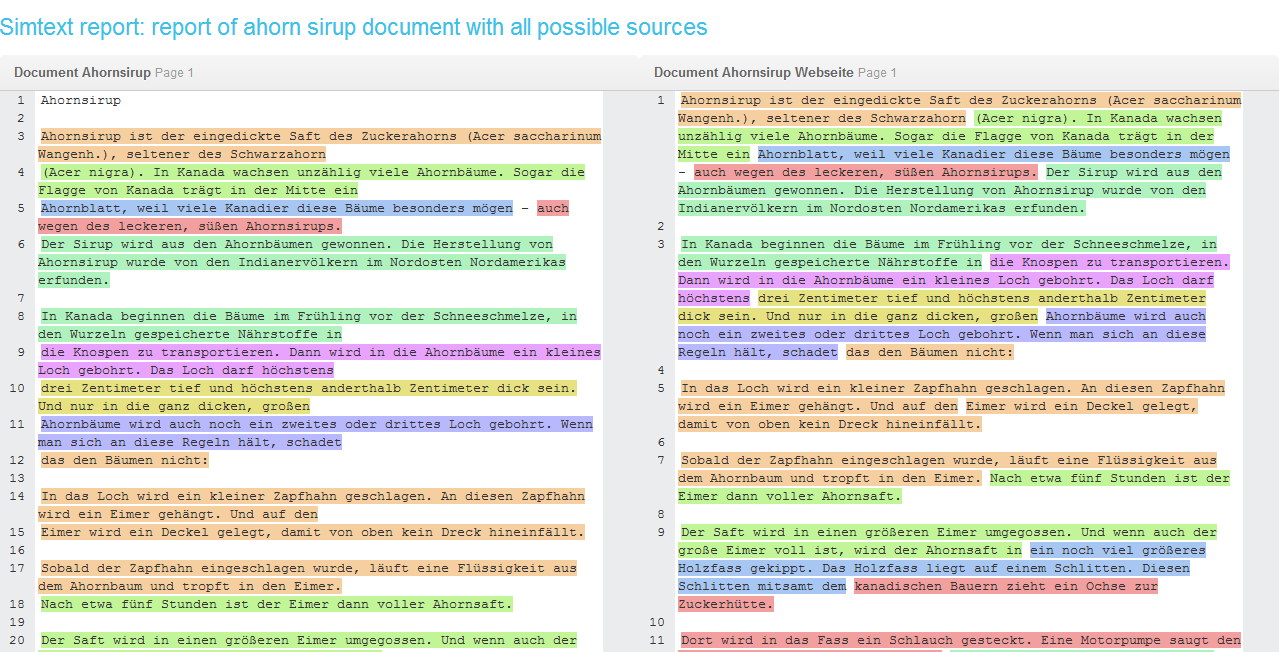
\includegraphics[width=0.97\textwidth]{images/sim_report_1.png}
  }
\fbox{
      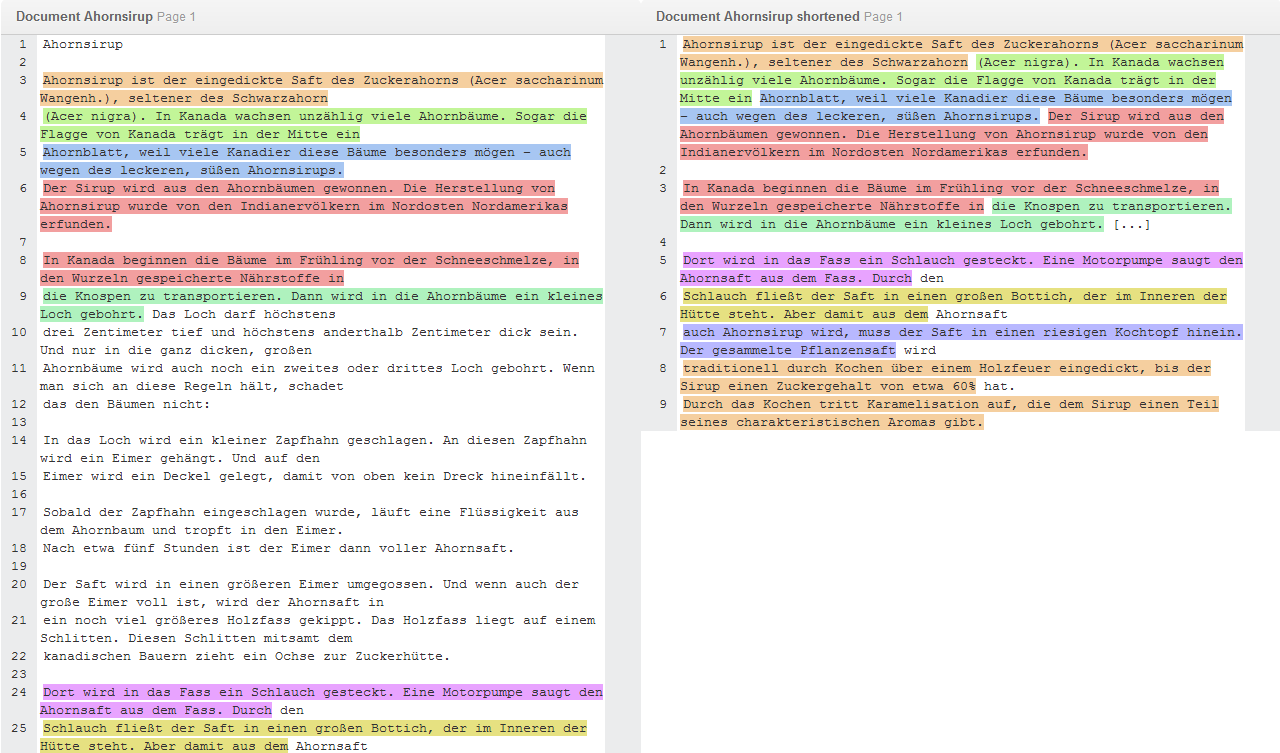
\includegraphics[width=0.97\textwidth]{images/sim_report_2.png}
  }
  \caption{Simtext of many documents}
  \label{fig:Simtext of many documents}
\end{figure}